\documentclass{beamer}
\usepackage{graphicx}
\usepackage{listings}

\lstdefinelanguage{Kotlin}{
comment=[l]{//},
commentstyle={\color{gray}\ttfamily},
emph={delegate, filter, first, firstOrNull, forEach, lazy, map, mapNotNull, println, return@},
emphstyle={\color{red}},
identifierstyle=\color{black},
keywords={abstract, actual, as, as?, break, by, class, companion, continue, data, do, dynamic, else, enum, expect, false, final, for, fun, get, if, import, in, interface, internal, is, null, object, operator, override, package, private, public, return, sealed, set, super, suspend, this, throw, true, try, typealias, val, var, vararg, when, where, while},
keywordstyle={\color{blue}\bfseries},
morecomment=[s]{/*}{*/},
morestring=[b]",
morestring=[s]{"""*}{*"""},
ndkeywords={@Deprecated, @JvmField, @JvmName, @JvmOverloads, @JvmStatic, @JvmSynthetic, Array, Byte, Double, Float, Int, Integer, Iterable, Long, Runnable, Short, String},
ndkeywordstyle={\color{Orange}\bfseries},
sensitive=true,
stringstyle={\color{green}\ttfamily},
showstringspaces=false,
}

\mode<presentation> { \usetheme{Madrid} }

\title{Kotlin\texorpdfstring{$\nabla$}{}}
\subtitle{Differentiable functional programming with algebraic data types}
\author{Breandan Considine}
\institute[UdeM]{
Universit\'e de Montr\'eal \\
\medskip
\textit{breandan.considine@umontreal.ca}
}
\date{\today}

\begin{document}
    \begin{frame}
        \titlepage
    \end{frame}

    \begin{frame}
        \frametitle{Overview}
        \tableofcontents
    \end{frame}

    \section{Introduction and motivation}\label{sec:first-section}

    \begin{frame}
        \frametitle{Kotlin}
        \begin{itemize}
            \item Goal: To implement automatic differentiation in Kotlin
            \item Kotlin is a JVM language with emphasis on type and null safety
            \item Offers features for building domain specific languages (DSLs)
            \item Supports first-class functions, higher order functions and FP
            \item Has support for extension functions and algebraic data types
            \item Operator overloading and other syntactic sugar (to be shown)
        \end{itemize}
    \end{frame}



    \begin{frame}
        \frametitle{Kotlin\texorpdfstring{$\nabla$}{}}
        \begin{itemize}
            \item
            \item Type system from algebraic first principles (group, ring, field)
            \item Automatic differentiation using a natural (infix) notation
            \item Supports partials and higher order derivatives, gradients
            \item Property-based testing using finite differences (Hypothesis, QuickCheck)
        \end{itemize}
    \end{frame}

    \section{A Short History of Computing Derivatives}\label{sec:second-section}

    %------------------------------------------------------------------------------------------------

        \begin{frame}
        \frametitle{Automatic differentiation}
        Suppose we have a program $P: \mathbb{R}\rightarrow\mathbb{R}$ where:
        %
        \begin{equation}
            P(x)=p_n \circ p_{n-1} \circ p_{n-2} \circ ... \circ p_1 \circ p_0
        \end{equation}
        %
        From the chain rule of calculus, we know that:
        %
        \begin{equation}
            \frac{dP}{dp_0} = {\displaystyle \prod_{i=1}^{n} \frac{dp_{i}}{dp_{i-1}}}
        \end{equation}
    \end{frame}


    %------------------------------------------------------------------------------------------------

    \begin{frame}
        \frametitle{Numerical differentiation}
        \begin{itemize}
            \item Many mathematical formula have discrete, numerical representations
            \item But numerical values can be an \textit{inexact} representation of math
            \item Long calculations on primitives are susceptible to rounding errors
            \item Bag of tricks for discrete approximation and numerical stability:
            \begin{itemize}
                \item Fourier, Chebyshev, Lagrange
                \item Arbitrary precision arithmetic
                \item Kahan summation algorithm
                \item log-sum-exp trick
            \end{itemize}
        \end{itemize}
    \end{frame}

    %------------------------------------------------------------------------------------------------

    \begin{frame}
        \frametitle{Symbolic differentiation}
        \begin{itemize}
            \item What about evaluating functions symbolically?
            \item Computer algebra systems for manipulate symbolic formulas
        \end{itemize}
    \end{frame}

    %------------------------------------------------------------------------------------------------

    %    \begin{frame}
    %        \frametitle{Automatic differentiation}
    %        \begin{itemize}
    %            \item Derivatives can be calculated automatically? (Wengert, 1964)
    %            \item Code as an \textit{exact} symbolic representation of functions
    %            \item To reason about code we need the ability to treat \textit{code as data}:
    %            \begin{itemize}
    %                \item Reflection and metaprogramming
    %                \item Domain specific languages
    %                \item First-class functions
    %            \end{itemize}
    %        \end{itemize}
    %    \end{frame}

    %------------------------------------------------------------------------------------------------

    %    \begin{frame}
    %        \frametitle{Differentiable [functional] programming}
    %        \begin{itemize}
    %            \item What is a program, but a series of arithmetic operations?
    %            \item What are arithmetic operations but syntactic sugar for functions?
    %            \item Functions can be composed of other functions or chained in sequence
    %            \item High school calculus gives us rules for differentiating function chains
    %            \item Pearlmutter \& Siskind teach us AD is possible just using FP (2016)
    %            \item Wang, Rompf, et al. show us this is possible \textit{without a tape}! (2018)
    %        \end{itemize}
    %    \end{frame}

    %------------------------------------------------------------------------------------------------

    %    \begin{frame}
    %        \frametitle{Differentiable programming with algebraic types}
    %        \begin{itemize}
    %            \item Combine the tools from mathematics and CS
    %            \item Type safety
    %            \item Static analysis
    %            \item Allows us to preserve symmetries that are not obvious
    %            \item There is an abstract algebra for tensor manipulations
    %            \item Can be encoded using OOP and parametric polymorphism
    %            \item \href{https://arxiv.org/pdf/1610.07690.pdf}{Operational Calculus for Differentiable Programming}
    %        \end{itemize}
    %    \end{frame}

    %------------------------------------------------------------------------------------------------


    \begin{frame}
        \frametitle{Not reinventing the wheel}
        \begin{itemize}
            \item Haskell already does this: Group
            \item Parsing expressions in a FP
        \end{itemize}
    \end{frame}

    %------------------------------------------------------------------------------------------------

    \section{Architectural Overview}\label{sec:third-section}

    \begin{frame}[fragile]
        \frametitle{Algebraic Data Types}
        \begin{lstlisting}[language=Kotlin, gobble=12]
            class Var: Expr()
            class Const(val num: Number): Expr()
            class Sum(val e1: Expr, val e2: Expr): Expr()
            class Prod(val e1: Expr, val e2: Expr): Expr()
            sealed class Expr: Group {
              fun diff() = when(expr) {
                is Const -> Zero
                is Sum -> e1.diff() + e2.diff()
                // d(u*v)/dx = du/dx * v + u * dv/dx
                is Prod -> e1.diff() * e2 + e1 * e2.diff()
                is Var -> One
              }
              operator fun plus(e: Expr) = Sum(this, e)
              operator fun times(e: Expr) = Prod(this, e)
            }
        \end{lstlisting}
    \end{frame}

    \begin{frame}[fragile]
        \frametitle{Expression Simplification}
        \begin{lstlisting}[language=Kotlin, gobble=12]
            operator fun Expr.times(e: Expr) = when {
              this is Const && num == 0.0 -> Const(0.0)
              this is Const && num == 1.0 -> exp
              exp is Const && exp.num == 0.0 -> exp
              exp is Const && exp.num == 1.0 -> this
              this is Const && exp is Const -> Const(num*exp.num)
              else -> Prod(this, e)
            }

            // Sum(Prod(Const(2.0), Var()), Const(6.0))
            val q = Const(2.0) * Sum(Var(), Const(3.0))
        \end{lstlisting}
    \end{frame}

    \begin{frame}[fragile]
        \frametitle{Testing}
        \begin{lstlisting}[language=Kotlin, gobble=12]
            val x = variable("x")
            val y = variable("y")

            val z = y * (sin(x * y) - x) // Function under test
            val dz_dx = d(z) / d(x)      // Automatic derivative
            val manualDx = y * (cos(x * y) * y - 1)

            "dz/dx should be y * (cos(x * y) * y - 1)" {
              assertAll (NumGen, NumGen) { cx, cy ->
                // Evaluate the results at a given seed
                val autoEval = dz_dx(x to cx, y to cy)
                val manualEval = manualDx(x to cx, y to cy)
                // Should pass if |adEval - manualEval| < eps
                autoEval shouldBeApproximately manualEval
              }
            }
        \end{lstlisting}
    \end{frame}

    \section{Usage}\label{sec:fourth-section}

    \begin{frame}[fragile]
        \frametitle{Usage}
        \begin{lstlisting}[language=Kotlin, gobble=12]
            with(DoubleFunctor) {// Use double-precision numerics
             val x = variable()  // Declare an immutable variable
             val y = sin(sin(sin(x)))/x + sin(x) * x + cos(x) + x

             // Lazily compute reverse-mode automatic derivatives
             val dy_dx = d(y) / d(x)
             val d2y_dx = d(dy_dx) / d(x)
             val d3y_dx = d(d2y_dx2) / d(x)
             val d4y_dx = d(d3y_dx3) / d(x)
             val d5y_dx = d(d4y_dx4) / d(x)

             plot(-10..10, dy_dx, dy2_dx, d3y_dx, d4y_dx, d5y_dx)
            }
        \end{lstlisting}
    \end{frame}

    \begin{frame}
        \frametitle{$y = \frac{\sin{\sin{\sin{x}}}}{x} + x \sin{x} + \cos{x} + x$, $\frac{dy}{dx}$, $\frac{d^{2}y}{dx^2}$, $\frac{d^{3}y}{dx^3}$, $\frac{d^{4}y}{dx^4}$, $\frac{d^{5}y}{dx^5}$}
        \begin{center}
            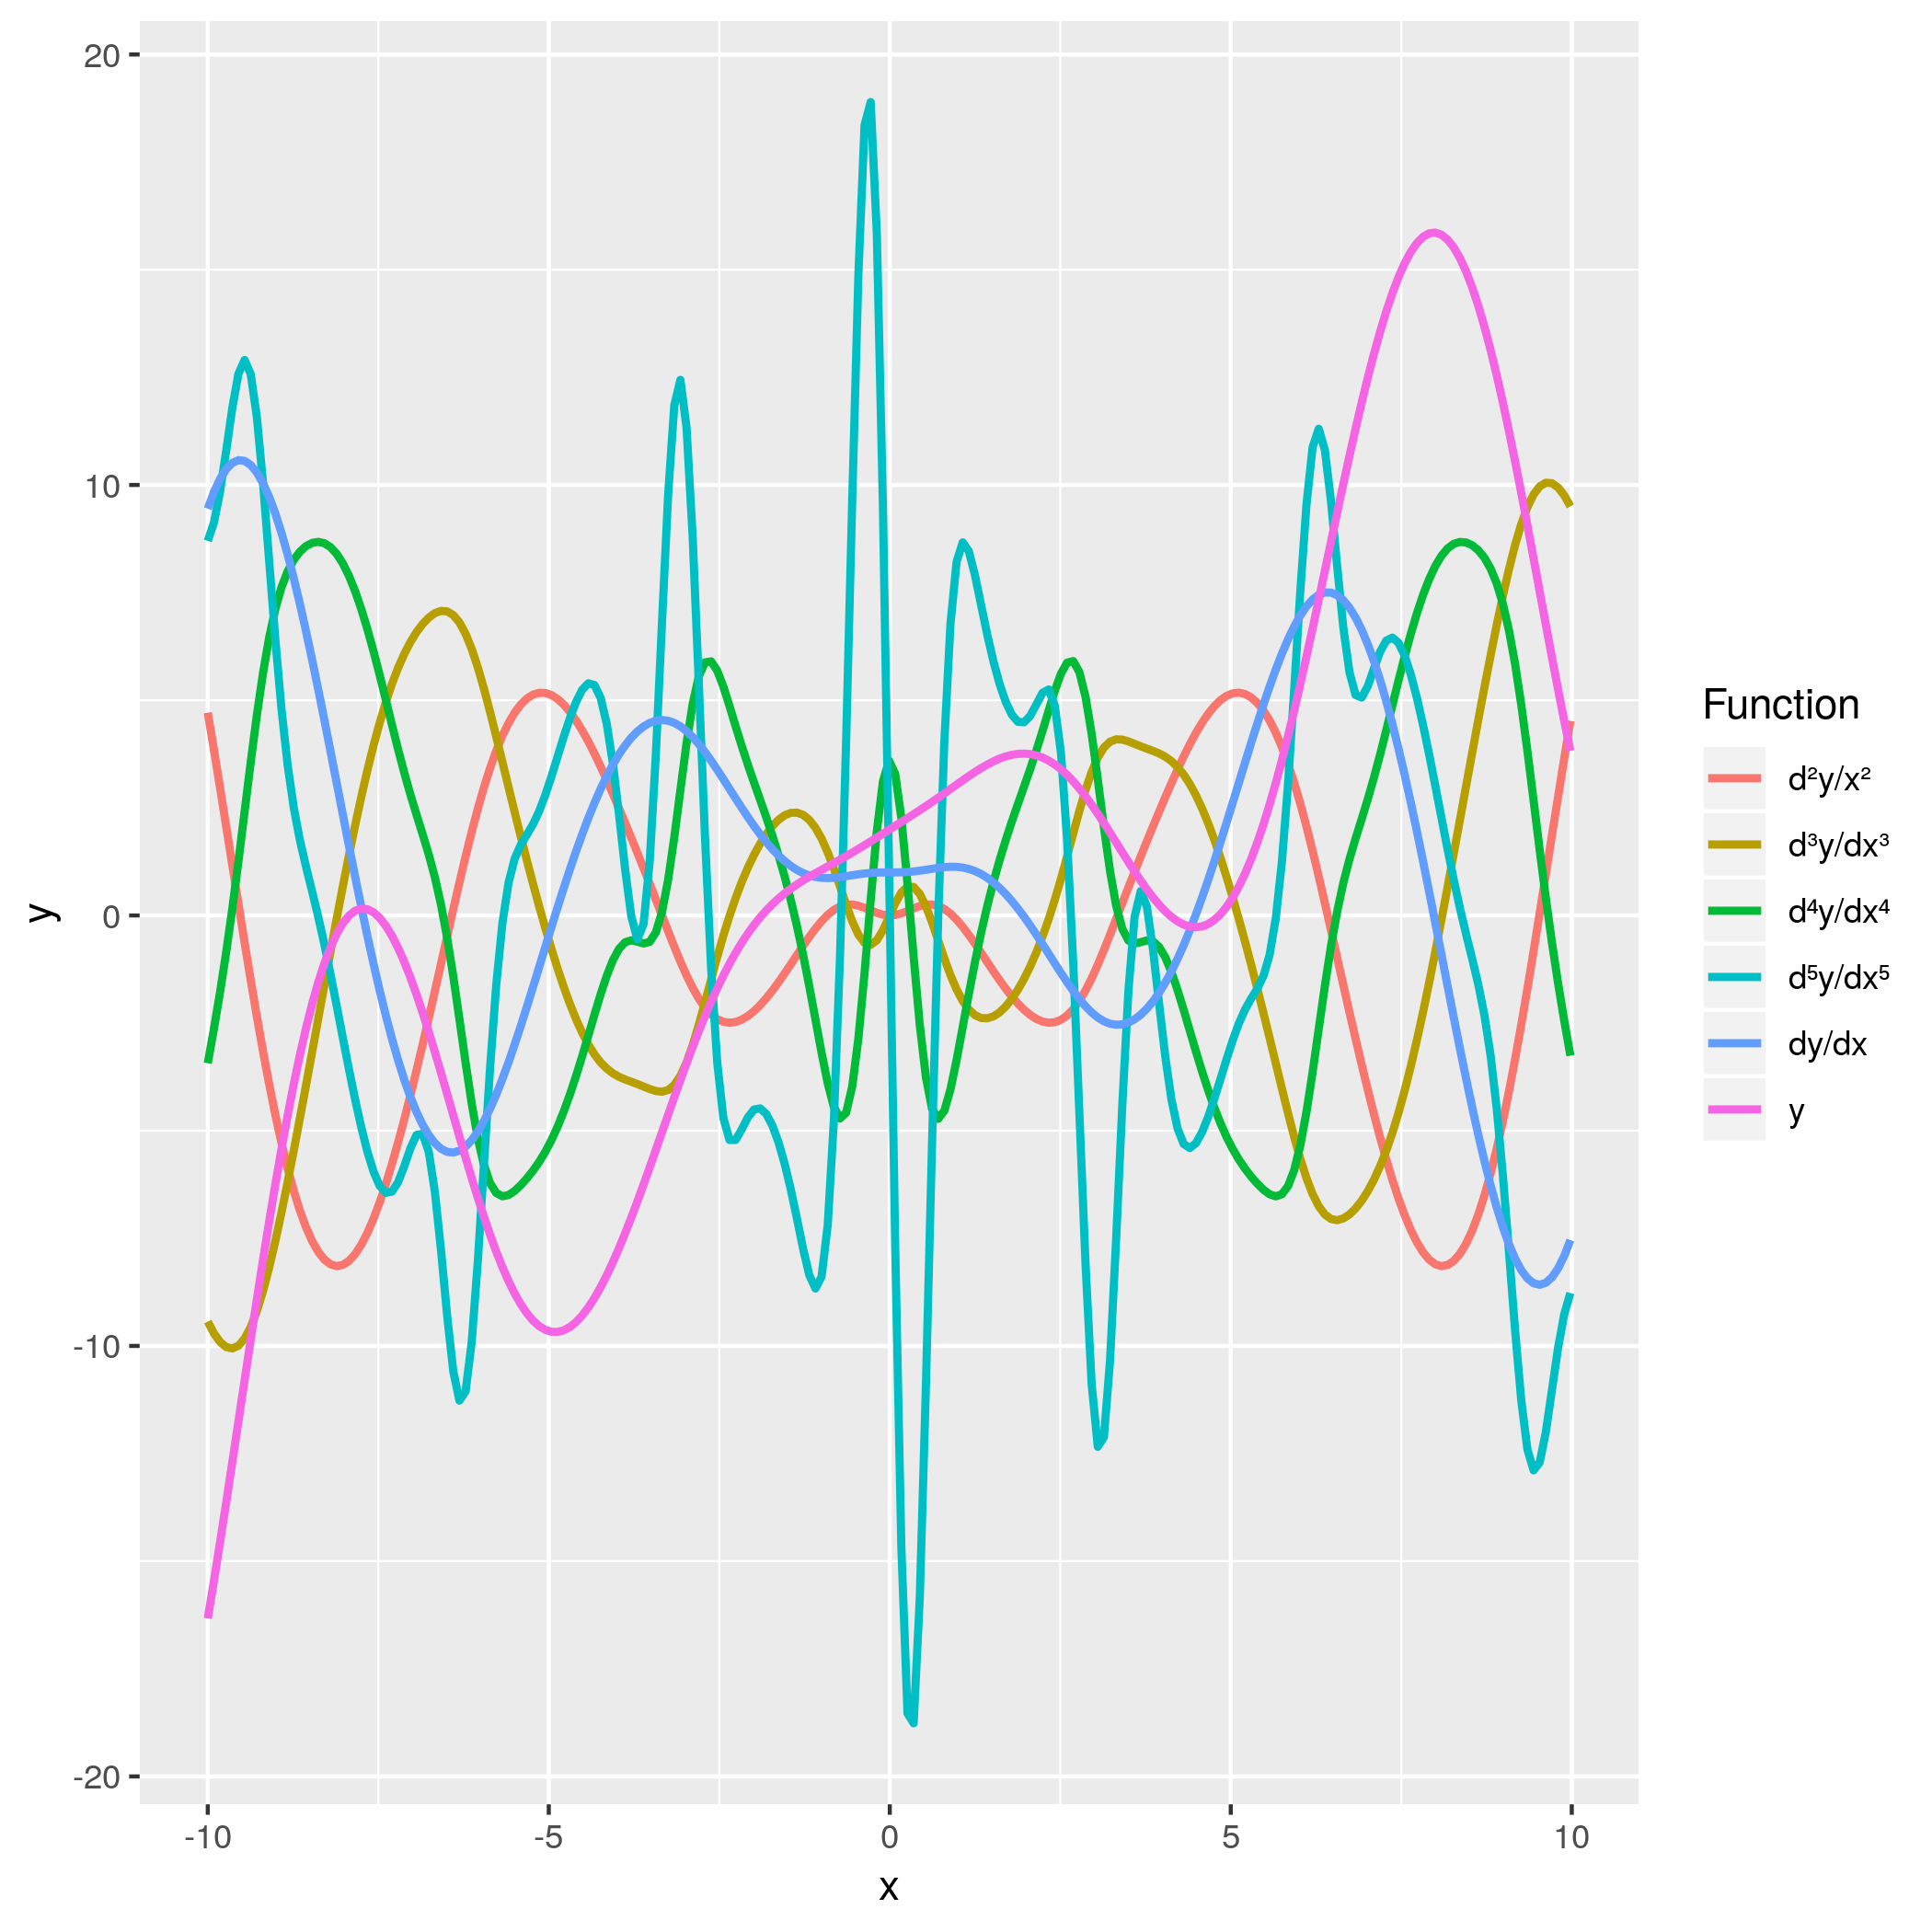
\includegraphics[scale=0.4]{plot.png}
        \end{center}
    \end{frame}

    \section{Future Plans}\label{sec:fifth-section}

    \begin{frame}
        \frametitle{Roadmap}
        \item TODO
    \end{frame}

    \begin{frame}
        \frametitle{Further directions to explore}
        \begin{itemize}
            \item Closer integration with Kotlin/Java standard library
            \item \href{https://discuss.kotlinlang.org/t/primitive-type-specialization/11022/4}{Primitive type specialization}
            \item Dependent types via code generation to type check tensor shapes
            \item Encode additional structure like arity into the type system
            \item Performance benchmarks and zero-cost un/boxing abstractions
            \item Lazy evaluation and configurable forward/backward AD modes
            \item Automatic expression refactoring for numerical stability
        \end{itemize}
    \end{frame}
\end{document}